% !TeX spellcheck = it_IT
\section{Introduzione}

\subsection{Scopo del documento}

Il presente documento ha l’intento di specificare la pianificazione delle attività che saranno svolte dai membri del gruppo Obelix per realizzare il progetto Monolith.

Gli scopi del presente documento sono:
\begin{itemize}
\item Analizzare i possibili fattori di rischio
\item Presentare la pianificazione delle attività e delle tempistiche
\item Preventivare l'utilizzo delle risorse necessarie allo svolgimento del progetto
\item Calcolare il consuntivo di utilizzo delle risorse durante l'evolversi dei lavori
\end{itemize}

\subsection{Scopo del prodotto}

Lo scopo del prodotto è quello di permettere la creazione di bolle
interattive, che dovranno funzionare nell’ambiente Rocket.chat. Queste
bolle permetteranno di aumentare l'interattività tra gli utenti della
chat e aggiungeranno nuove funzionalità accessibili
direttamente dalla conversazione senza il bisogno di ricorrere
all'apertura di applicazioni diverse.
Il sistema offrirà agli sviluppatori un set di \glossario{API} per creare e
rilasciare nuove bolle e agli utenti finali la possibilità di
usufruire di un insieme di bolle predefinite.

\subsection{Glossario}

Al fine di evitare ogni ambiguità di linguaggio e massimizzare la
comprensione dei documenti, i termini che necessitano di essere
chiariti saranno scritti in corsivo e marcati con una |G| alla prima
occorrenza in pedice e
saranno riportati nel \gloss.

\subsection{Riferimenti}

\subsubsection{Normativi}
\begin{itemize}
\item \textbf{Norme di Progetto}: \\ \normediprogetto
\item \textbf{Capitolato d'appalto C5}: \\ \url{http://www.math.unipd.it/~tullio/IS-1/2016/Progetto/C5.pdf}
\item \textbf{Regolamento del progetto didattico}: \\ \url{http://www.math.unipd.it/~tullio/IS-1/2016/Dispense/L09.pdf}
\item \textbf{Vincoli di organigramma e dettagli tecnico-economici}: \\ \url{http://www.math.unipd.it/~tullio/IS-1/2016/Progetto/PD01b.html}

\end{itemize}


\subsubsection{Informativi}
\begin{itemize}
\item \textbf{Slide del corso di Ingegneria del Software}: \\  \url{http://www.math.unipd.it/~tullio/IS-1/2016/ }
\end{itemize}

\subsection{Modello di sviluppo}

Il modello di sviluppo scelto è il Modello Incrementale. Esso prevede la suddivisione dello svolgimento del progetto in più periodi il cui termine è segnato da una \textit{milestone}:

\begin{itemize}
	\item \textbf{Analisi preliminare}: inizialmente avviene la ricerca degli strumenti utili per redigere la documentazione. Successivamente si definiscono i documenti relativi alle normative e alle scelte interne. Come ultima parte vengono redatti i documenti riguardanti le scelte strategiche, qualitative e di analisi del progetto.
	\item \textbf{Analisi di Dettaglio}: in questo periodo avviene un miglioramento dell'analisi dei requisiti. Gli analisti correggono gli eventuali requisiti che non rispecchiano le aspettative del \glossario{proponente} e ne trovano di nuovi.
	\item \textbf{Progettazione architetturale e di Dettaglio}: durante lo svolgimento della Progettazione architetturale si individua una soluzione generale per soddisfare i requisiti richiesti. Verranno inoltre sistemati ed incrementati gli altri documenti.
	\item \textbf{Codifica e test}: questo periodo termina con la Revisione di Qualifica. Qui viene svolta la codifica dei requisiti obbligatori, opzionali e desiderabili. Verranno incrementati altri documenti. 
	\item \textbf{Validazione e collaudo}: in questo periodo il progetto raggiunge la sua terminazione. Viene effettuata l'attività di validazione del software e successivo collaudo. Questo periodo termina con la Revisione  di Accettazione. 
\end{itemize}

Il Modello Incrementale prevede che:
\begin{itemize}
\item L’Analisi e la Progettazione Architetturale costituiscano una base solida: i requisiti e l’architettura del sistema sono identificati e fissati definitivamente e sono essenziali per la pianificazione dei cicli incrementali
\item La Progettazione di Dettaglio, la codifica e i test vengano ripetuti più volte, permettendo sia il miglioramento di parti del sistema già esistenti che l’aggiunta di nuove funzionalità
\end{itemize}

I vantaggi attesi dalla scelta di tale modello sono i seguenti:

\begin{itemize}
\item I requisiti utente sono organizzati in base all'importanza strategica, ovvero vengono soddisfatti per primi quelli di maggiore rilevanza
\item Ogni incremento può produrre valore e riduce il rischio di fallimento, in quanto esso
consolida ulteriormente la base ed eventualmente ne aumenta la qualità
\item Minimizza i rischi di ritardo rispetto ai tempi stabiliti dato che le fasi hanno durata breve e sono precedentemente pianificate
\item Attività di verifica più semplice
\item Rilasci multipli e in successione, che inizialmente punteranno a soddisfare i requisiti di primaria importanza mentre successivamente andranno ad adempiere a possibili funzionalità aggiuntive o opzionali.
\item Il favoreggiamento della creazione di prototipi, ovvero di parti di prodotto funzionanti, che a loro volta favoriscono
il dialogo con il cliente.

\end{itemize}



\subsection{Scadenze}

Il gruppo Obelix ha deciso di rispettare le seguenti scadenze:

\begin{itemize}

\item Revisione dei Requisiti: 2017-04-18
\item Revisione di Progettazione: 2017-06-20
\item Revisione di Qualifica: 2017-08-29
\item Revisione di Accettazione: 2017-09-12

\end{itemize}

\section{Analisi dei rischi}
In questa sezione verranno elencati i possibili rischi a cui il gruppo di lavoro Obelix potrebbe andare incontro nella realizzazione di Monolith.\\Per poterli gestire è stata utilizzata la seguente procedura:
\begin{itemize}
\item \textbf{Identificazione dei rischi}: individuazione dei potenziali rischi che possono presentarsi durante il ciclo di vita del prodotto e classificazione secondo la loro natura:
  \begin{itemize}
  \item Rischi tecnologici\item Rischi organizzativi\item Rischi sul personale\item Rischi sulla strumentazione\item Rischi sui requisiti
  \end{itemize}

\item \textbf{Analisi dei rischi}: di ogni rischio si studieranno:
  \begin{itemize}
  \item Probabilità di occorrenza (Molto bassa, bassa, media, alta, molto alta)\item Livello di gravità
  \end{itemize}

\item \textbf{Pianificazione di controllo}: istituire metodi di controllo dei  rischi, così da poterli evitare
\item \textbf{Mitigazione}: istituire un piano di contingenza per
  mitigare gli effetti deleteri di un rischio nel caso questo
  dovesse verificarsi. Tale fase è richiesta solo per rischi
  difficilmente controllabili e gestibili
\end{itemize}

\subsection{Rischi tecnologici}
\subsubsection{Tecnologie adottate}

\begin{center}
	
	\begin{tabular}{|>{\centering}m{4cm} ||>{\centering}m{8cm} |>{\centering\arraybackslash}m{0pt}@{}|}
		\hline
		\textbf{Descrizione} & Quasi tutte le tecnologie adottate dal \glossario{team} sono sconosciute ai suoi membri & \\[2ex]
		\hline	
		\textbf{Probabilità} & Alta &\\[1ex]
		\hline
		\textbf{Livello di gravità} & Serio & \\[1ex]
		\hline
		\textbf{Conseguenze} & Allungamento dei tempi dovuto all'apprendimento delle nozioni necessarie per il progetto & \\[1ex]
		\hline
		\textbf{Trattamento} & Ogni componente del gruppo deve, in maniera autonoma, studiare tutte le tecnologie necessarie per la realizzazione del prodotto facendo uso dei documenti forniti dall’\emph{Amministratore} & \\[1ex] 
		\hline
		\textbf{Riscontri} & Il team si è adoperato per uno studio personale delle tecnologie da adottare senza causare ritardi eccessivi sui tempi di consegna stimati & \\[1ex]
		\hline
	\end{tabular}
	
\end{center}

%\begin{itemize}
%\item \textbf{Descrizione}: quasi tutte le tecnologie adottate dal \glossario{team} sono sconosciute ai suoi membri\item \textbf{Probabilità}: Alta
%\item \textbf{Livello di gravità}: Serio
%\item \textbf{Conseguenze}: Grosso rallentamento nello sviluppo del prodotto finale
%\item \textbf{Trattamento}: Ogni componente del gruppo deve, in maniera autonoma, studiare tutte le tecnologie necessarie per la realizzazione del prodotto facendo uso dei documenti forniti dall’ \emph{Amministratore} 
%\item \textbf{Attualizzazione nel periodo}:
%  \begin{itemize}
%  \item \textbf{Analisi dei requisiti}: il rischio non si è ancora verificato dato che non sono state
%    usate tali tecnologie in questo periodo di sviluppo
%  \end{itemize}
%\end{itemize}

\subsubsection{Guasti Hardware}
Ogni componente del gruppo possiede un computer portatile, da ciò deriva il rischio di un guasto tecnico ad uno o più computer.

\begin{center}
	
	\begin{tabular}{|>{\centering}m{4cm} ||>{\centering}m{8cm} |>{\centering\arraybackslash}m{0pt}@{}|}
		\hline
		\textbf{Descrizione} & Si verifica un guasto hardware che comporta la perdita di dati & \\[2ex]
		\hline	
		\textbf{Probabilità} & Bassa &\\[1ex]
		\hline
		\textbf{Livello di gravità} & Medio & \\[1ex]
		\hline
		\textbf{Conseguenze} & La perdita di dati comporterà la ripetizione del lavoro per ricreare il materiale perso. Questo porterà a un ritardo di entità proporzionale alla perdita & \\[1ex]
		\hline
		\textbf{Trattamento} & Ogni membro del gruppo possiede un altro dispositivo per poter continuare il lavoro in caso di malfunzionamenti o rotture hardware & \\[1ex] 
		\hline
		\textbf{Riscontri} & Fino ad ora il problema non si è presentato & \\[1ex]
		\hline
	\end{tabular}
	
\end{center}


\subsection{Rischi organizzativi}
\subsubsection{Rotazione ruoli}

\begin{center}
	
	\begin{tabular}{|>{\centering}m{4cm} ||>{\centering}m{8cm} |>{\centering\arraybackslash}m{0pt}@{}|}
		\hline
		\textbf{Descrizione} & I membri del gruppo dovranno scambiarsi i vari ruoli cambiando, di volta in volta, i propri compiti e responsabilità & \\[2ex]
		\hline	
		\textbf{Probabilità} & Bassa &\\[1ex]
		\hline
		\textbf{Livello di gravità} & Medio & \\[1ex]
		\hline
		\textbf{Conseguenze} & Si può verificare un rallentamento nello sviluppo del prodotto e/o un abbassamento della qualità di esso & \\[1ex]
		\hline
		\textbf{Trattamento} & La rotazione dei ruoli viene prestabilita, dando così modo ad ogni membro del gruppo di prepararsi anticipatamente per ricoprire il ruolo che gli verrà assegnato & \\[1ex] 
		\hline
		\textbf{Riscontri} & Dopo un approccio iniziale con piccole difficoltà il team non ha riscontrato problemi nella rotazione dei ruoli  & \\[1ex]
		\hline
	\end{tabular}
	
\end{center}
\newpage
\subsubsection{Pianificazione errata}

\begin{center}
	
	\begin{tabular}{|>{\centering}m{4cm} ||>{\centering}m{8cm} |>{\centering\arraybackslash}m{0pt}@{}|}
		\hline
		\textbf{Descrizione} & Durante la pianificazione è possibile che i tempi per l’esecuzione di alcune attività vengano calcolati in modo errato & \\[2ex]
		\hline	
		\textbf{Probabilità} & Media &\\[1ex]
		\hline
		\textbf{Livello di gravità} & Alto & \\[1ex]
		\hline
		\textbf{Conseguenze} & Una sottostima provocherà ritardi e slittamenti; una sovrastima porterà invece a uno spreco del tempo disponile per le attività di progetto & \\[1ex]
		\hline
		\textbf{Trattamento} & Si è deciso di prevedere, per ogni attività, un periodo maggiore di quanto normalmente richiesto, in modo tale che un eventuale ritardo non influenzi la durata totale del progetto & \\[1ex] 
		\hline
		\textbf{Riscontri} & Si sono verificati alcuni errori nella pianificazione che hanno portato ad un ritardo sui tempi di consegna inizialmente previsti & \\[1ex]
		\hline
	\end{tabular}
	
\end{center}

\subsection{Rischi sul personale}
\subsubsection{Problemi dei componenti del gruppo}

\begin{center}
	
	\begin{tabular}{|>{\centering}m{4cm} ||>{\centering}m{8cm} |>{\centering\arraybackslash}m{0pt}@{}|}
		\hline
		\textbf{Descrizione} & Ogni membro del gruppo ha impegni e necessità proprie. Di conseguenza diventa inevitabile
		il verificarsi di problemi organizzativi in seguito a
		sovrapposizioni di tali impegni con le attività del gruppo & \\[2ex]
		\hline	
		\textbf{Probabilità} & Media &\\[1ex]
		\hline
		\textbf{Livello di gravità} & Medio & \\[1ex]
		\hline
		\textbf{Conseguenze} & Si possono verificare problemi nella pianificazione e di conseguenza ritardi sulla consegna dei materiali & \\[1ex]
		\hline
		\textbf{Trattamento} & Quando possibile, ogni membro del
		gruppo si impegna a segnalare in anticipo la propria assenza, in
		modo da ricalcolare i tempi stimati per le varie attività. Sarà
		compito del  \emph{Responsabile}  di Progetto, riassegnare i compiti
		utilizzando la piattaforma di gestione delle attività & \\[1ex] 
		\hline
		\textbf{Riscontri} & Nonostante varie difficoltà nel organizzare incontri con il gruppo al completo è stato comunque effettuato un buon lavoro di programmazione per sopperire a questo problema & \\[1ex]
		\hline
	\end{tabular}
	
\end{center}

\newpage
\subsubsection{Problemi tra i componenti del gruppo}

\begin{center}
	
	\begin{tabular}{|>{\centering}m{4cm} ||>{\centering}m{8cm} |>{\centering\arraybackslash}m{0pt}@{}|}
		\hline
		\textbf{Descrizione} & Per tutti i componenti del gruppo,
		quest’attività di progetto è la prima esperienza in un gruppo
		così numeroso. Tale fattore potrebbe causare problemi di
		collaborazione causando squilibri interni, provocando così dei
		ritardi nei lavori e un clima non proficuo & \\[2ex]
		\hline	
		\textbf{Probabilità} & Bassa &\\[1ex]
		\hline
		\textbf{Livello di gravità} & Alto & \\[1ex]
		\hline
		\textbf{Conseguenze} & Nel caso in cui il rischio si verifichi, l’ambiente di lavoro può diventare pesante e non cooperativo, causando il ritardo nelle attività di progetto & \\[1ex]
		\hline
		\textbf{Trattamento} & Il \emph{Responsabile}  provvederà ad affidare
		alle persone coinvolte delle attività che non le faccia
		lavorare assieme, ripristinando così il clima corretto per
		svolgere in modo idoneo le attività nei tempi stabiliti & \\[1ex] 
		\hline
		\textbf{Riscontri} & Questo rischio non si è ancora verificato & \\[1ex]
		\hline
	\end{tabular}
	
\end{center}

\subsubsection{Problemi di inesperienza}

\begin{center}
	
	\begin{tabular}{|>{\centering}m{4cm} ||>{\centering}m{8cm} |>{\centering\arraybackslash}m{0pt}@{}|}
		\hline
		\textbf{Descrizione} & Per ogni componente del gruppo è la
		prima esperienza con questo metodo di lavoro. Sono richieste dell
		capacità di pianificazione e di analisi che il gruppo ancora non
		possiede. Inoltre è richiesto l’utilizzo di strumenti mai
		incontrati prima e alcune tecnologie richiedono del tempo per
		essere apprese & \\[2ex]
		\hline	
		\textbf{Probabilità} & Alta &\\[1ex]
		\hline
		\textbf{Livello di gravità} & Alto & \\[1ex]
		\hline
		\textbf{Conseguenze} & L'inesperienza del gruppo può portare a prendere delle decisioni sbagliate e/o un allungamento dei tempi dovuto all'apprendimento delle nozioni necessarie per il progetto & \\[1ex]
		\hline
		\textbf{Trattamento} & Ogni membro del gruppo si impegna a
		studiare il materiale necessario per l’utilizzo delle tecnologie e
		degli strumenti richiesti durante lo svolgimento del progetto. Nel
		caso in cui questo non fosse sufficiente il  \emph{Responsabile}  dovrà
		preparare un piano di studi per sopperire ad ogni tipo di lacuna & \\[1ex] 
		\hline
		\textbf{Riscontri} & Il rischio si è presentato portando alcuni ritardi sulla consegna prevista in precedenza & \\[1ex]
		\hline
	\end{tabular}
	
\end{center}

\subsection{Rischi sulla strumentazione}
\subsubsection{Inesperienza nell'utilizzo degli strumenti}

\begin{center}
	
	\begin{tabular}{|>{\centering}m{4cm} ||>{\centering}m{8cm} |>{\centering\arraybackslash}m{0pt}@{}|}
		\hline
		\textbf{Descrizione} & Molti degli strumenti software adottati dal gruppo per l’attività di progetto risultano essere inediti & \\[2ex]
		\hline	
		\textbf{Probabilità} & Media & \\[1ex]
		\hline
		\textbf{Livello di gravità} & Medio & \\[1ex]
		\hline
		\textbf{Conseguenze} & Ne deriva un rallentamento delle attività
		che sfruttano di questi strumenti & \\[1ex]
		\hline
		\textbf{Trattamento} & Nel caso di difficoltà a padroneggiare uno
		strumento, è compito del  \emph{Responsabile}  di Progetto assegnare
		ulteriore personale all’apprendimento di esso. Nel caso in cui,
		anche dopo tale intervento, non risulti essere possibile
		padroneggiare lo strumento, allora si dovrà adottare un altro
		strumento & \\[1ex] 
		\hline
		\textbf{Riscontri} & Molti strumenti adottati erano già conosciuti ai membri del team rendendo minore il tempo di apprendimento dedicato ai restanti sconosciuti & \\[1ex]
		\hline
	\end{tabular}
	
\end{center}

\subsection{Rischi sui requisiti}
\subsubsection{Incomprensione dei requisiti}

\begin{center}
	
	\begin{tabular}{|>{\centering}m{4cm} ||>{\centering}m{8cm} |>{\centering\arraybackslash}m{0pt}@{}|}
		\hline
		\textbf{Descrizione} & Può capitare che, data l’inesperienza del gruppo nell’affrontare l’analisi dei requisiti e nel capire le nuove tecnologie adottate dal capitolato, alcuni requisiti vengano compresi in modo errato & \\[2ex]
		\hline	
		\textbf{Probabilità} & Bassa & \\[1ex]
		\hline
		\textbf{Livello di gravità} & Alto & \\[1ex]
		\hline
		\textbf{Conseguenze} & Ne deriva una divergenza tra la visione
		del prodotto da parte del gruppo di progetto e le aspettative del
		proponente. Di conseguenza, in caso il proponente non sia d’accordo,
		sarà necessario rivisitare ciascun requisito e la relativa
		implementazione & \\[1ex]
		\hline
		\textbf{Trattamento} & In caso di dubbi sui requisiti sarà il  \emph{Responsabile}  a organizzare, nel modo descritto nelle \normediprogetto, un incontro (o un semplice contatto) con i proponenti in modo tale da risolvere ogni dubbio & \\[1ex] 
		\hline
		\textbf{Riscontri} & Il problema non si è ancora verificato in quanto il team ha concordato ogni decisione da prendere con i proponenti  & \\[1ex]
		\hline
	\end{tabular}
s	
\end{center}



\section{Pianificazione}
Il gruppo ha deciso di suddividere lo sviluppo del progetto in sei periodi di lavoro:

\begin{itemize}
\item Analisi dei Requisiti(AR)
\item Analisi dei Requisiti in Dettaglio (AD)
\item Progettazione Architetturale(PA)
\item Progettazione di Dettaglio (PD)
\item Codifica(CO)
\item Validazione (VA)
\end{itemize}

Per ogni periodo viene presentato un diagramma di Gantt.
All'interno dei diagrammi le \glossario{milestone} vengono rappresentate con dei rombi neri.
Ogni periodo termina con una milestone che può essere esterna e coincidere con le
date di consegna dei documenti, oppure interna e dipendere da scadenze concordate
dal gruppo.
La durata di ogni attività è mostrata da linee nere, le cui estremità sono
delle frecce rivolte verso il basso. Ogni attività è suddivisa in sotto-attività.
Le sotto-attività possono essere critiche o non critiche.

\begin{itemize}
\item \textbf{Critiche}: hanno un forte impatto temporale sull’intero progetto.
  Il ritardo di una di queste attività risulterebbe particolarmente dannoso per
  l’efficienza del gruppo di lavoro e causerebbe un ritardo nel raggiungimento della
  milestone.
  Sono indicate nel diagramma con il colore rosso
\item \textbf{Non critiche}: possono essere svolte parallelamente alle sotto-attività critiche.
  Un ritardo in tali attività non comporta uno slittamento temporale di tutto il progetto.
  Sono indicate nel diagramma con il colore verde
\end{itemize}

\subsection{Analisi dei Requisiti}

\begin{sidewaysfigure}
  \centering
  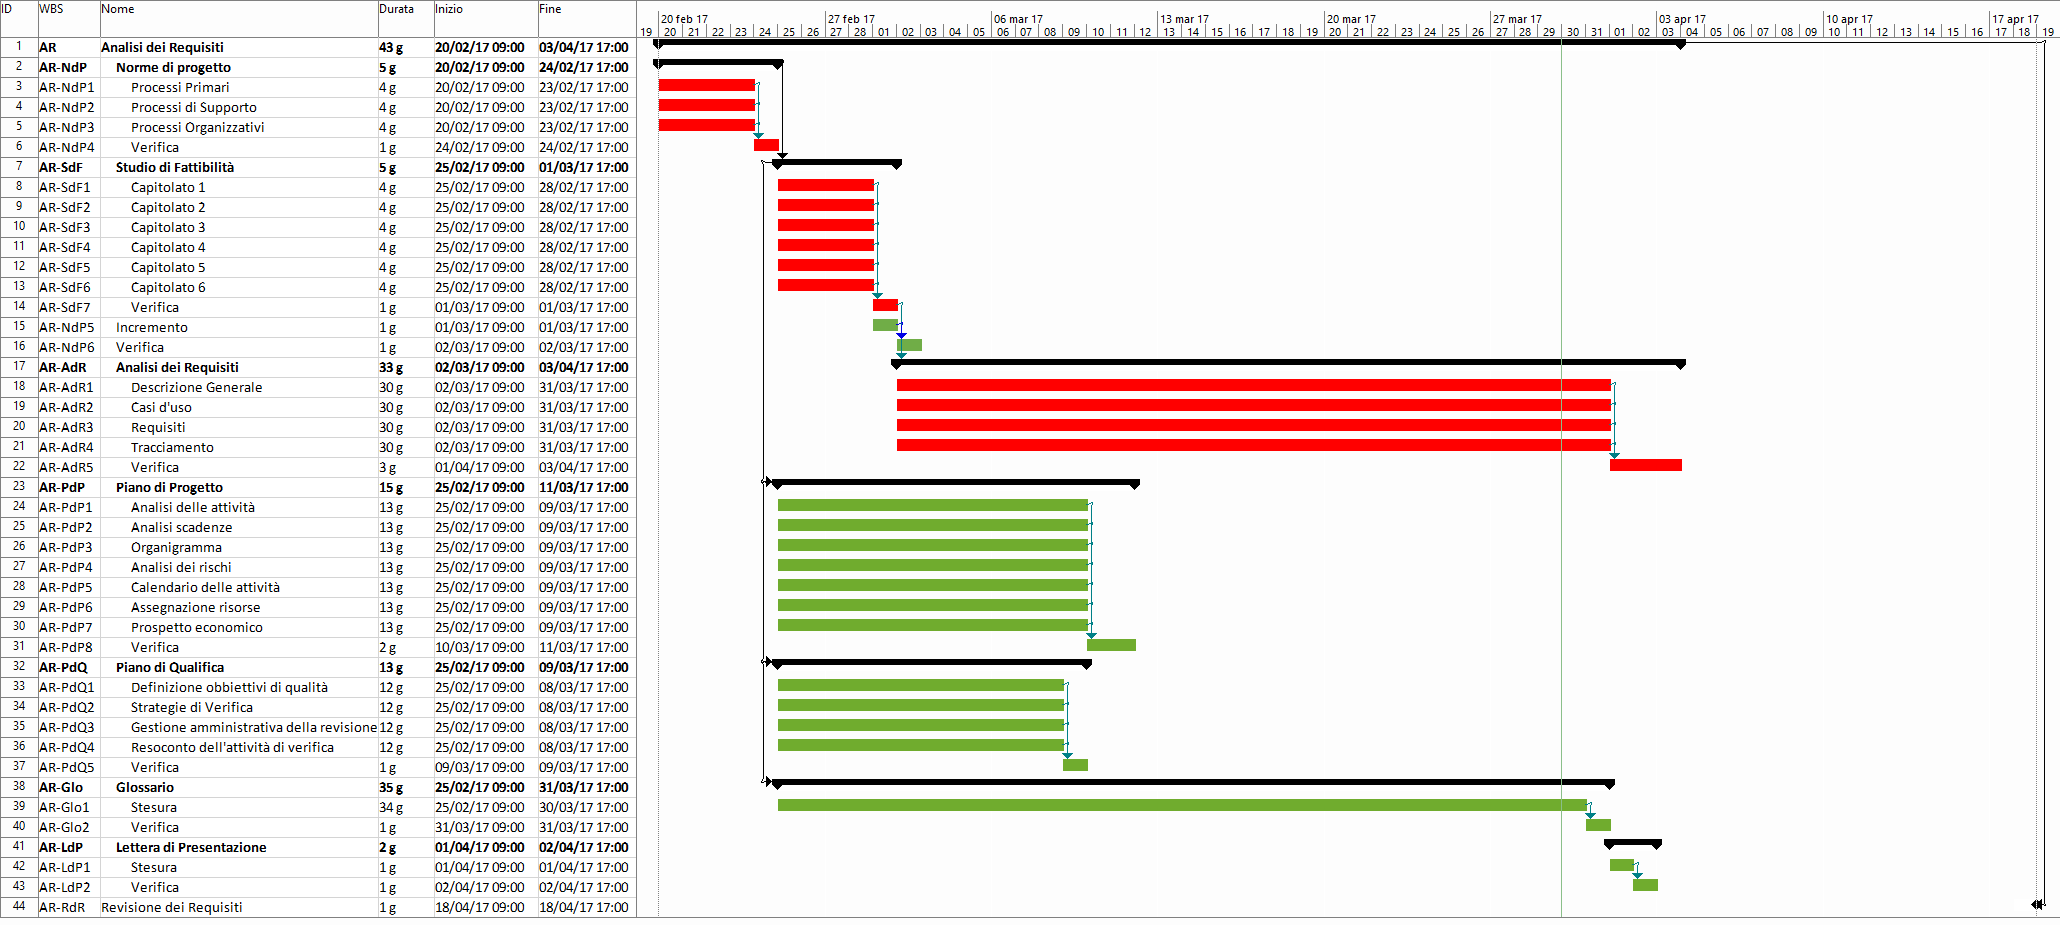
\includegraphics[scale=0.28]{img/1-AR.png}
  \captionof{figure}{Diagramma di Gantt relativo al periodo di Analisi dei Requisiti}
\end{sidewaysfigure}

Periodo: da 2017-02-20 a 2017-04-18 \\
Questo periodo inizia in concomitanza alla formazione del gruppo e termina con la Revisione dei Requisiti. Il gruppo deve scegliere un capitolato e cominciare a lavorare con il fine ultimo di aggiudicarselo.\\
I documenti che saranno stilati in questo periodo sono:

\begin{itemize}
\item \textbf{Norme di Progetto}: l’ \emph{Amministratore}  si occupa di stilare questo documento
  inserendovi le norme che il gruppo dovrà seguire durante lo svolgimento di tutte
  le attività. \'E un'attività critica perché sono stabilite anche le norme
  che regolano la stesura di tutti gli altri documenti

\item \textbf{Studio di Fattibilità}: gli  \emph{Analisti}  analizzano tutti i capitolati valutandone
  i fattori positivi e negativi. \'E un'attività critica perché porterà alla scelta del
  progetto sul quale il gruppo andrà a lavorare. Deve precedere, dunque, l'Analisi dei
  Requisiti

\item \textbf{Analisi dei Requisiti}: Gli  \emph{Analisti}  approfondiscono l'analisi del capitolato
  scelto

\item \textbf{Piano di Progetto}: il  \emph{Responsabile}  di Progetto organizza le attività assegnandole
  alle risorse disponibili. Tale attività ha alta priorità in quanto regola le attività
  svolte dall’intero gruppo

\item \textbf{Piano di Qualifica}: i  \emph{Verificatori}  definiscono come devono essere effettuate le
  verifiche al fine di consegnare un prodotto di qualità

\item \textbf{Glossario}: tutti i redattori dei documenti contribuiscono alla stesura del
  Glossario in modo incrementale. Contiene la spiegazione di alcuni termini, al fine di
  eliminare ogni ambiguità di significato.

\item \textbf{Lettera di Presentazione}: il gruppo dichiara di voler partecipare alla gara d'appalto

\end{itemize}

Dopo essere stati redatti, tutti i documenti verranno  verificati. La verifica dei
documenti è considerata un'attività critica.\\
In questa periodo i ruoli maggiormente coinvolti sono:  \emph{Amministratore} ,  \emph{Responsabile} ,
 \emph{Analista}  e  \emph{Verificatore} .

\subsection{Analisi dei Requisiti in Dettaglio}

\begin{center}
  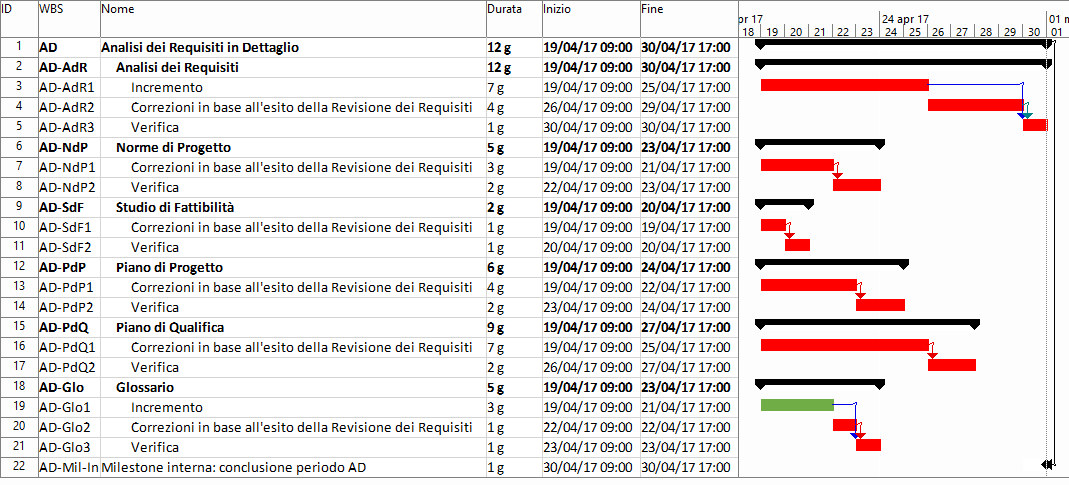
\includegraphics[scale=0.3]{img/2-AD.png}
  \captionof{figure}{Diagramma di Gantt relativo al periodo di Analisi dei Requisiti in Dettaglio}
\end{center}

Periodo: da 2017-04-19 a 2017-04-30 \\
Questo periodo inizia dopo la Revisione dei Requisiti e termina con l’inizio del periodo
successivo, quello di Progettazione Architetturale.
Il gruppo in questo periodo si impegnerà ad identificare, ampliare e fissare definitivamente i requisiti richiesti dal sistema.
Verranno inoltre effettuate le modifiche necessarie, rilevate in seguito all’esito della Revisione dei Requisiti nei vari documenti. \\
In questa periodo i ruoli maggiormente coinvolti sono:  \emph{Analista}  e  \emph{Verificatore} .

\subsection{Progettazione Architetturale}

\begin{center}
  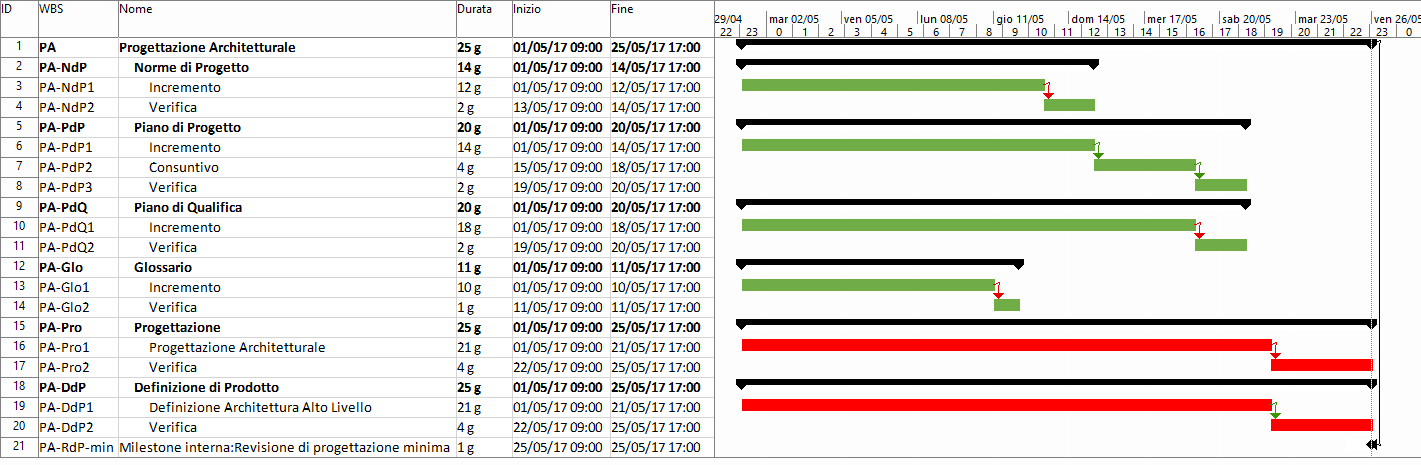
\includegraphics[scale=0.25]{img/3-PA.png}
  \captionof{figure}{\small Diagramma di Gantt relativo al periodo di Progettazione Architetturale}
\end{center}

Periodo: da 2017-05-01 a 2017-05-25 \\
Il periodo di Progettazione Architetturale inizia dopo quello di Analisi dei Requisiti
in Dettaglio e si conclude con la milestone interna di Revisione di Progettazione minima.
L’obiettivo di questo periodo è la stesura della progettazione ad alto livello del sistema.
\'E prevista la stesura delle sezioni del documento Definizione di Prodotto riguardanti l'Architettura di alto livello. 
I Progettisti dovranno descrivere le scelte progettuali, i design-pattern scelti per la realizzazione dell’architettura generale del prodotto, i principali flussi di controllo e il tracciamento dei requisiti. \\
In questa fase i ruoli maggiormente coinvolti sono:  \emph{Amministratore} ,  \emph{Responsabile} ,
 \emph{Progettista}  e  \emph{Verificatore} . \\

\subsection{Progettazione di Dettaglio}

\begin{center}
  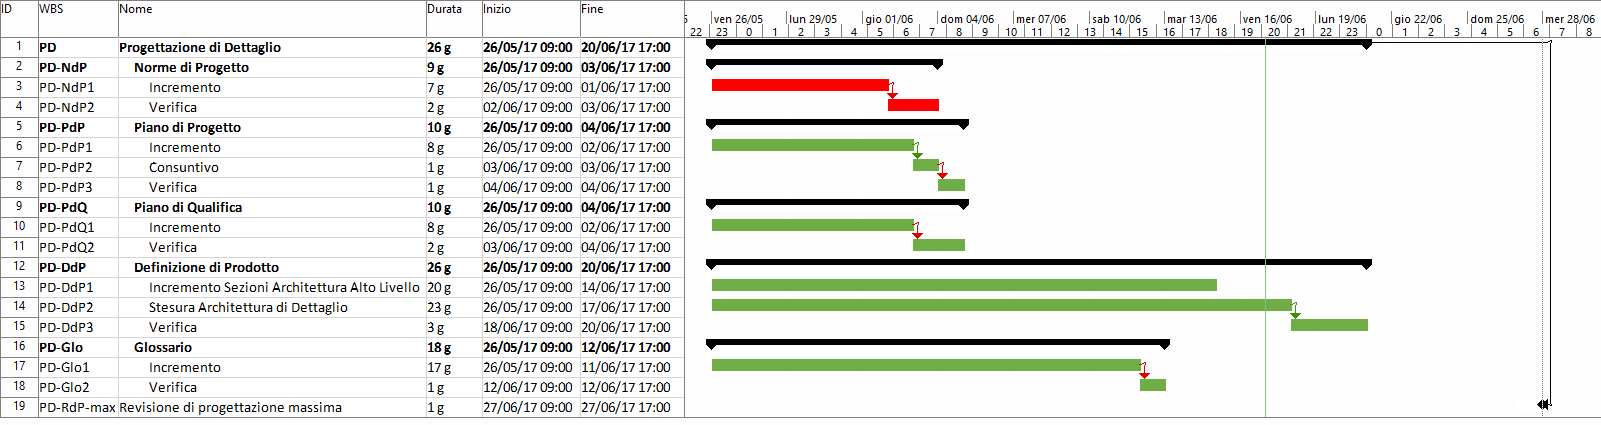
\includegraphics[scale=0.2]{img/4-PD.png}
  \captionof{figure}{Diagramma di Gantt relativo al periodo di Progettazione di Dettaglio}
\end{center}

Periodo: da 2017-05-26 a 2017-06-20 \\
Il periodo di Progettazione in Dettaglio inizia dopo quello di Progettazione Architetturale
e si conclude con la scadenza di consegna per la Revisione di Progettazione massima.
L’obiettivo di questo periodo è la progettazione dettagliata del sistema.
\'E prevista la stesura delle sezioni del documento Definizione di Prodotto riguardanti l'architettura di dettaglio del sistema.
I Progettisti dovranno descrivere le classi per ogni componente del sistema, i design-pattern scelti per la realizzazione dell’architettura di dettaglio del prodotto e il tracciamento dei requisiti. \\
In questa fase i ruoli maggiormente coinvolti sono:  \emph{Amministratore} ,  \emph{Responsabile} ,
 \emph{Progettista}  e  \emph{Verificatore} .

\subsection{Codifica}

\begin{center}
  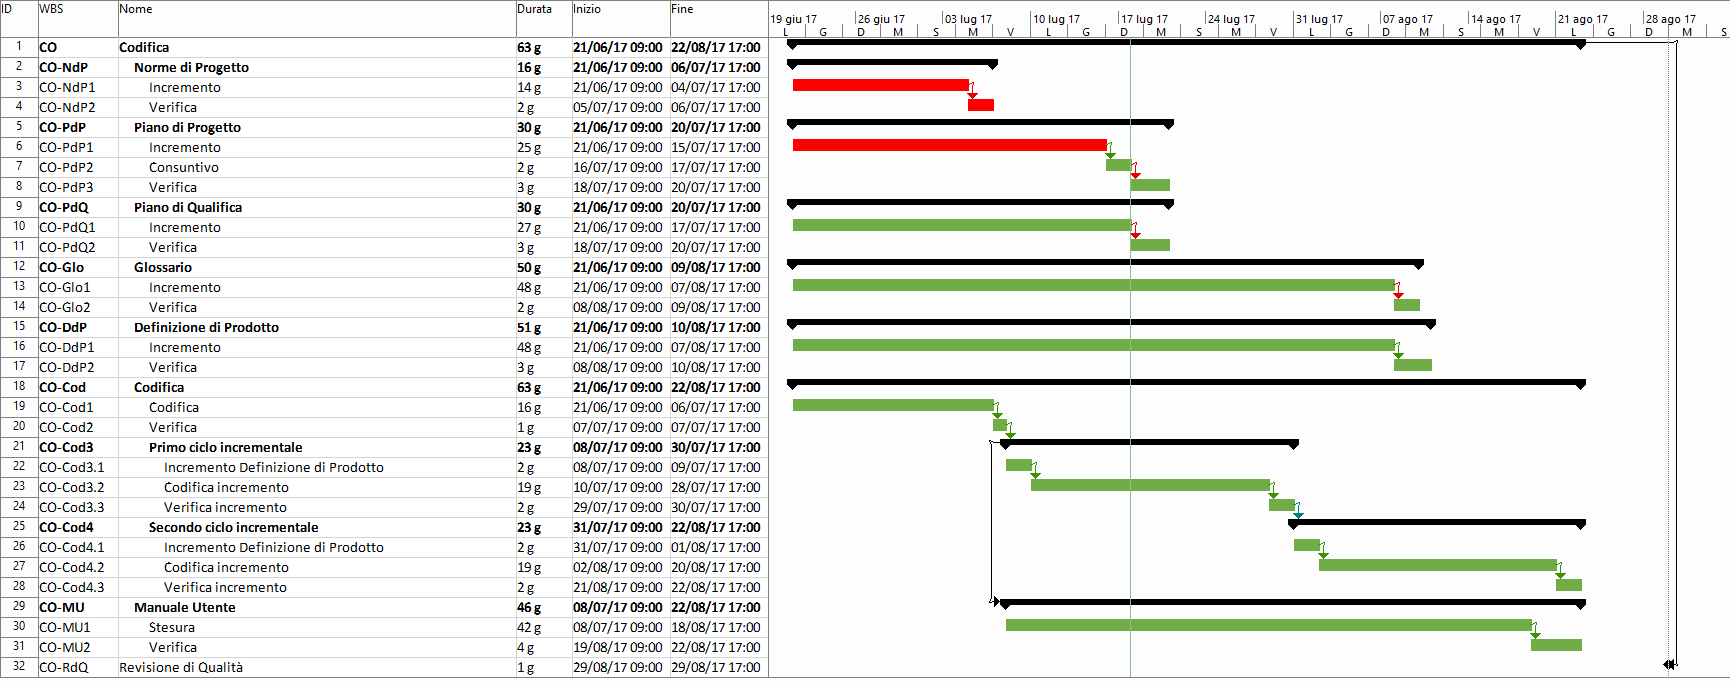
\includegraphics[scale=0.23]{img/5-CO.png}
  \captionof{figure}{Diagramma di Gantt relativo al periodo di Codifica}
\end{center}

Periodo: da 2017-06-21 a 2017-08-22 \\
Il periodo di Codifica inizia dopo quello di Progettazione in Dettaglio e si conclude
con la consegna del prodotto per la Revisione di Qualifica. 
\'E prevista la realizzazione incrementale del prodotto, ovvero verranno realizzati prima i requisiti essenziali, poi quelli desiderabili e infine quelli facoltativi per ridurre il rischio di fallimento.
L’obiettivo finale consiste nel consegnare un prodotto software completo. Le attività che ad ogni incremento verranno eseguite sono le seguenti:
\begin{itemize}
	\item Aggiornare il documento Definizione di Prodotto
	\item Incrementare i documenti Norme di Progetto, Piano di Progetto, Piano di Qualifica e Glossario.
	\item I Programmatori devono sviluppare il codice del prodotto software attenendosi il più possibile a quanto scritto dai Progettisti nel documento Definizione di Prodotto. \\
    L’attività di Codifica deve essere svolta seguendo, iterativamente, i seguenti passi:
    \begin{itemize}
    	\item Codifica dell’incremento svolto dai Progettisti
    	\item Verifica dell’incremento
	\end{itemize}
	\item Stesura del Manuale Utente
\end{itemize}

In questa fase i ruoli maggiormente coinvolti sono:  \emph{Amministratore} ,  \emph{Responsabile} ,
 \emph{Progettista} ,  \emph{Programmatore}  e  \emph{Verificatore} .

\subsection{Validazione}

\begin{center}
  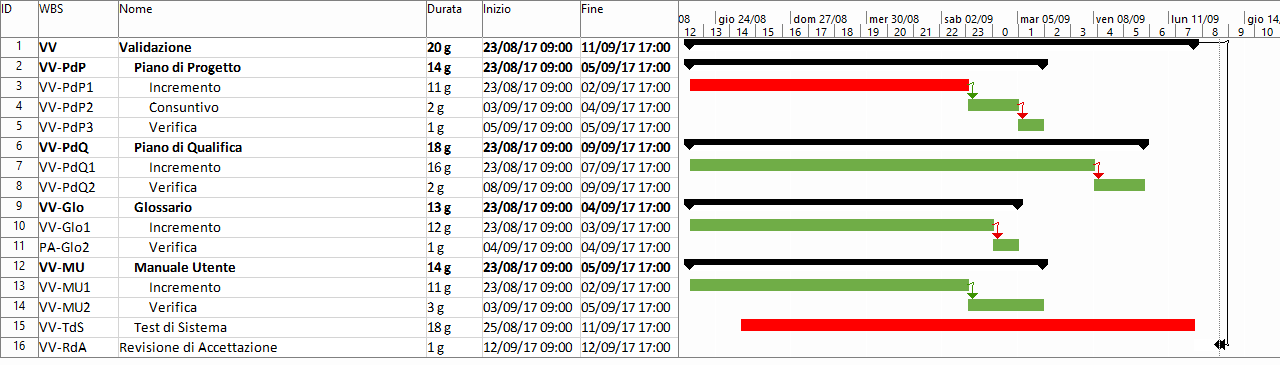
\includegraphics[scale=0.18]{img/6-VA.png}
  \captionof{figure}{Diagramma di Gantt relativo al periodo di Validazione}
\end{center}

Periodo: da 2017-08-23 a 2017-09-12 \\
Il periodo di Validazione inizia dopo quello di Codifica e si conclude con la Revisione
di Accettazione.
L'obbiettivo di questo periodo è quello di effettuare tutti i test necessari per garantire
che il prodotto soddisfi tutti i requisiti. 
Le attività previste per questo periodo sono:
\begin{itemize}
\item Effettuare i test di sistema
\item Incrementare, correggere o aggiornare e verificare i documenti: Manuale Utente, Norme di Progetto, Piano di Progetto, Piano di Qualifica, Definizione di Prodotto e Glossario
\item Verificare il corretto funzionamento del prodotto correggendo eventuali errori
\end{itemize}

In questa fase i ruoli maggiormente coinvolti sono:  \emph{Responsabile} ,  \emph{Progettista} 
e  \emph{Verificatore} .

\section{Calendario delle attività}
In questa sezione vengono presentati i quadri riassuntivi ed i grafici dell’impegno dei ruoli nei diversi periodi. Infine vengono mostrate le incidenze dei vari ruoli nell’intero progetto.


\subsection{Analisi dei Requisiti}
Le ore impiegate in questo periodo sono 195 e vengono ripartite in:
\begin{center}
  \centering
  \begin{tabular}{|c|c|}
    \hline
    \textbf{Ruolo} & \textbf{Ore} \\
    \hline
     \emph{Responsabile}  & 40 \\
    \hline  \emph{Amministratore}  & 20 \\
    \hline  \emph{Analista}  & 80 \\
    \hline  \emph{Verificatore}  & 55 \\
    \hline
  \end{tabular}
  \captionof{table}{Ore a ruolo, Analisi dei Requisiti}
  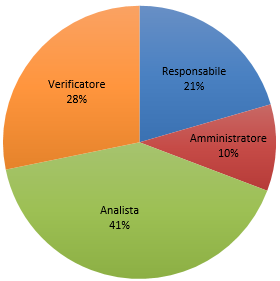
\includegraphics[scale=0.7]{img/grafico1.png}
  \captionof{figure}{Incidenza ore per ruolo, Analisi dei Requisiti}
\end{center}




\subsection{Analisi dei requisiti in dettaglio}
Le ore impiegate in questo periodo sono 96 e vengono ripartite in:

\begin{center}
  \centering
  \begin{tabular}{|c|c|}
    \hline
    \textbf{Ruolo} & \textbf{Ore} \\
    \hline
     \emph{Responsabile}  & 20 \\
    \hline  \emph{Amministratore}  & 20 \\
    \hline  \emph{Analista}  & 34 \\
    \hline  \emph{Verificatore}  & 22 \\
    \hline
  \end{tabular}
  \captionof{table}{Ore a ruolo, Analisi dei Requisiti}
  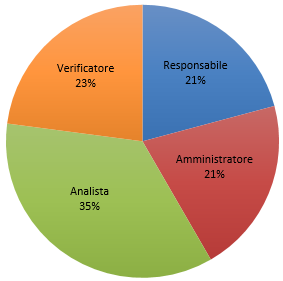
\includegraphics[scale=0.7]{img/grafico2.png}
  \captionof{figure}{Incidenza ore per ruolo, Analisi dei Requisiti in dettaglio}
\end{center}



\subsection{Progettazione Architetturale}
Le ore impiegate in questo periodo sono 140 e vengono ripartite in:
\begin{center}
  \centering
  \begin{tabular}{|c|c|}
    \hline
    \textbf{Ruolo} & \textbf{Ore} \\
    \hline
     \emph{Responsabile}  & 22 \\
    \hline  \emph{Amministratore}  & 14 \\
    \hline  \emph{Progettista}  & 71 \\
    \hline  \emph{Verificatore}  & 33 \\
    \hline
  \end{tabular}
  \captionof{table}{Ore a ruolo, Progettazione Architetturale}
  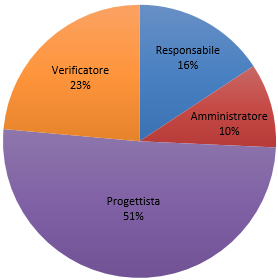
\includegraphics[scale=0.7]{img/grafico3.png}
  \captionof{figure}{Incidenza ore per ruolo, Progettazione Architetturale}
\end{center}



\subsection{Progettazione di Dettaglio}
Le ore impiegate in questo periodo sono 135 e vengono ripartite in:
\begin{center}
  \centering
  \begin{tabular}{|c|c|}
    \hline
    \textbf{Ruolo} & \textbf{Ore} \\
    \hline
     \emph{Responsabile}  & 17 \\
    \hline  \emph{Amministratore}  & 12 \\
    \hline  \emph{Progettista}  & 70 \\
    \hline  \emph{Verificatore}  & 36 \\
    \hline
  \end{tabular}
  \captionof{table}{Ore a ruolo, Progettazione di Dettaglio}
  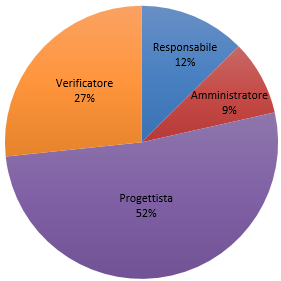
\includegraphics[scale=0.7]{img/grafico4.png}
  \captionof{figure}{Incidenza ore per ruolo, Progettazione di Dettaglio}
\end{center}

\subsection{Codifica}
Le ore impiegate in questo periodo sono 220 e vengono ripartite in:
\begin{center}
  \centering
  \begin{tabular}{|c|c|}
    \hline
    \textbf{Ruolo} & \textbf{Ore} \\
    \hline
     \emph{Responsabile}  & 13 \\
    \hline  \emph{Amministratore}  & 6 \\
    \hline  \emph{Progettista}  & 20 \\
    \hline  \emph{Programmatore}  & 118 \\
    \hline  \emph{Verificatore}  & 63 \\
    \hline
  \end{tabular}
  \captionof{table}{Ore a ruolo, Codifica}
  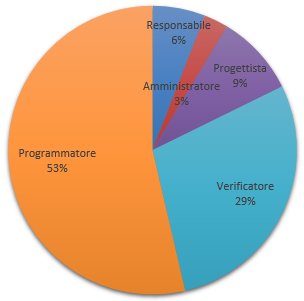
\includegraphics[scale=0.7]{img/grafico5.png}
  \captionof{figure}{Incidenza ore per ruolo, Codifica}
\end{center}

\subsection{Validazione}
Le ore impiegate in questo periodo sono 144 e vengono ripartite in:
\begin{center}
  \centering
  \begin{tabular}{|c|c|}
    \hline
    \textbf{Ruolo} & \textbf{Ore} \\
    \hline
     \emph{Responsabile}  & 26 \\
    \hline  \emph{Progettista}  & 35 \\
    \hline  \emph{Verificatore}  & 83 \\
    \hline
  \end{tabular}
  \captionof{table}{Ore a ruolo, Validazione}
  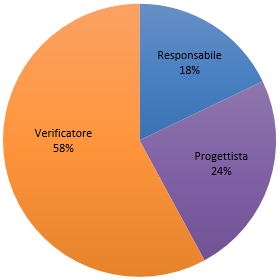
\includegraphics[scale=0.7]{img/grafico6.png}
  \captionof{figure}{Incidenza ore per ruolo, Validazione}
\end{center}

\subsection{Quadro riassuntivo}
Le ore totali del progetto sono 930, di cui 639 remunerabili, così ripartite:
\begin{center}
  \centering
  \begin{tabular}{|c|c|c|}
    \hline
    \textbf{Ruolo} & \textbf{Ore totali} & \textbf{Ore remunerabili} \\
    \hline
     \emph{Responsabile}  & 138 & 78 \\
    \hline  \emph{Amministratore}  & 72 & 32 \\
    \hline  \emph{Progettista}  & 196 & 196 \\
    \hline  \emph{Programmatore}  & 118 & 118 \\
    \hline  \emph{Analista}  & 114 & 0 \\
    \hline  \emph{Verificatore}  & 292 & 215 \\
    \hline
  \end{tabular}
  \captionof{table}{Ore a ruolo, Quadro riassuntivo}
  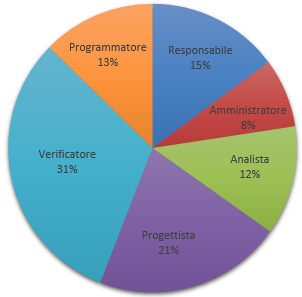
\includegraphics[scale=0.7]{img/grafico7.png}
  \captionof{figure}{Incidenza ore per ruolo, Ore Totali}
  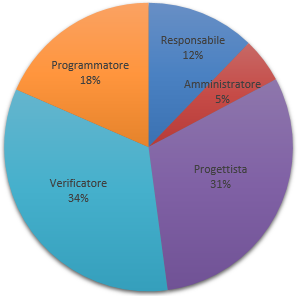
\includegraphics[scale=0.7]{img/grafico8.png}
  \captionof{figure}{Incidenza ore per ruolo, Ore Rendicontate}
\end{center}

\section{Suddivisione del lavoro}
A turno, ogni membro del gruppo dovrà rivestire i panni di tutti i
ruoli specificati nell'organigramma. Durante le varie fasi
ogni componente può ricoprire più ruoli, anche contemporaneamente,
purché non si creino conflitti di alcun genere nello svolgimento delle
attività. 

\subsection{Analisi dei requisiti}
Nell’attività di Analisi dei Requisiti ciascun componente dovrà rivestire i seguenti ruoli:

\begin{center}
  \centering
  \begin{tabular} {|c|c|c|c|c|c|c|c|}
    \hline
    \textbf{Nominativo} & \multicolumn{6}{|c|}{\textbf{Ore per ruolo}} & \textbf{Ore Totali} \\
    & \textbf{Re} & \textbf{Am} & \textbf{An} & \textbf{Pj} & \textbf{Pr} & \textbf{Ve} & \\
    \hline
    Emanuele Crespan & & 15 & 17 & & & & 32\\
    \hline
    Tomas Mali &  & 5 & 8 & & & 20 & 33\\
    \hline
    Silvio Meneguzzo & & & 17 & & & 15 & 32\\
    \hline
    Nicolò Rigato & 20 & & 13 & & &  & 33\\
    \hline
    Riccardo Saggese & & & 12 & & & 20 & 32\\
    \hline
    Federica Schifano & 20 & & 13 & & & & 33\\
    \hline
  \end{tabular}
  \captionof{table}{Ore per componente, Analisi dei Requisiti}
  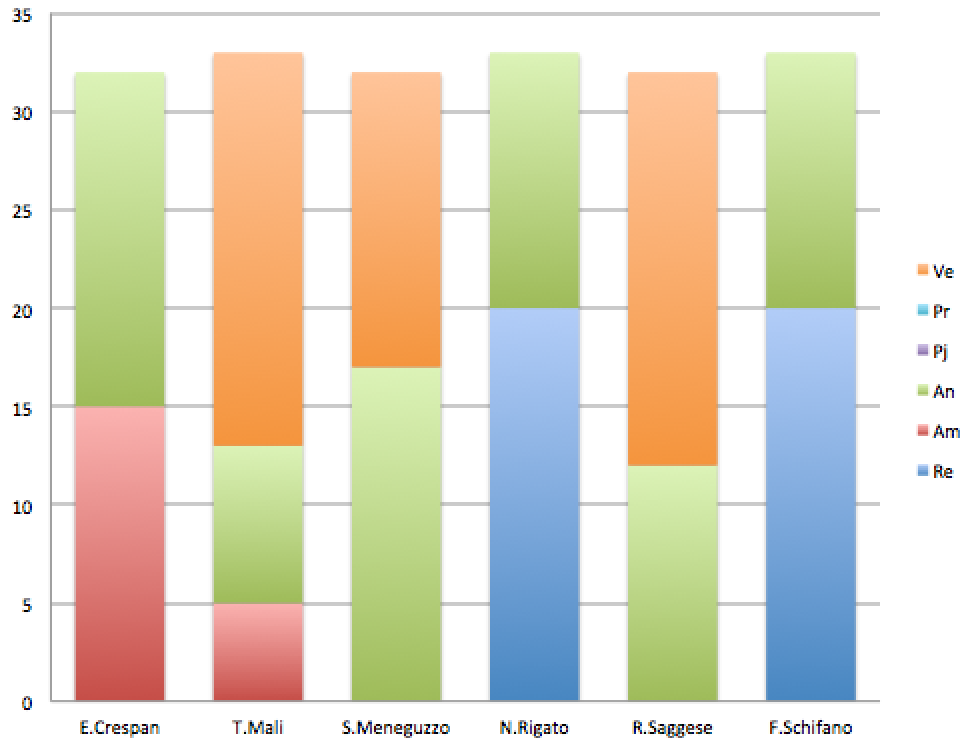
\includegraphics[scale=0.65]{img/fig1.png}
  \captionof{figure}{Incidenza ore per ruolo, Analisi dei requisiti}
\end{center}

\subsection{Analisi dei Requisiti in Dettaglio}
Nell’attività di Analisi dei Requisiti in Dettaglio ciascun componente dovrà rivestire i seguenti ruoli:
\begin{center}
  \centering
  \begin{tabular} {|c|c|c|c|c|c|c|c|}
    \hline
    \textbf{Nominativo} & \multicolumn{6}{|c|}{\textbf{Ore per ruolo}} & \textbf{Ore Totali} \\
    & \textbf{Re} & \textbf{Am} & \textbf{An} & \textbf{Pj} & \textbf{Pr} & \textbf{Ve} & \\
    \hline
    Emanuele Crespan & &10 &6 & & & &16 \\
    \hline
    Tomas Mali &10 & &6 & & & &16 \\
    \hline
    Silvio Meneguzzo & & &5 & & &11 &16\\
    \hline
    Nicolò Rigato &10 & &6 & & & &16\\
    \hline
    Riccardo Saggese & &10 &6 & & & &16\\
    \hline
    Federica Schifano & & &5 & & &11 &16\\
    \hline
  \end{tabular}
  \captionof{table}{Ore per componente, Analisi dei Requisiti in dettaglio}
  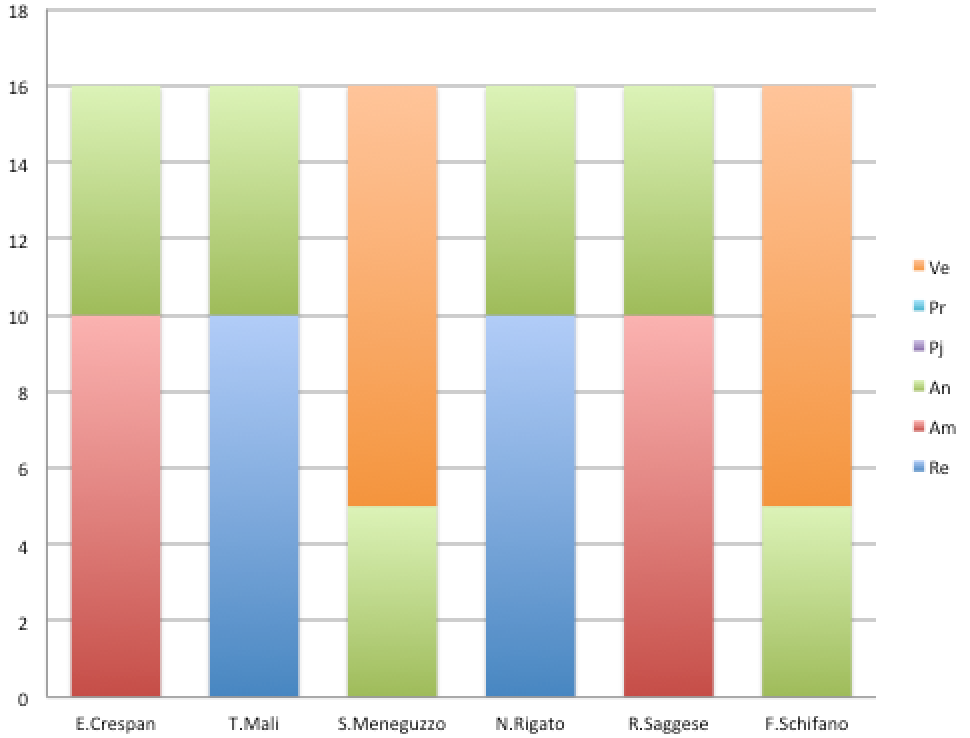
\includegraphics[scale=0.65]{img/fig2.png}
  \captionof{figure}{Incidenza ore per ruolo, Analisi dei requisiti in dettaglio}
\end{center}

\subsection{Progettazione architetturale}
Nell’attività di Progettazione architetturale ciascun componente dovrà rivestire i seguenti ruoli:
\begin{center}
  \centering
  \begin{tabular} {|c|c|c|c|c|c|c|c|}
    \hline
    \textbf{Nominativo} & \multicolumn{6}{|c|}{\textbf{Ore per ruolo}} & \textbf{Ore Totali} \\
    & \textbf{Re} & \textbf{Am} & \textbf{An} & \textbf{Pj} & \textbf{Pr} & \textbf{Ve} & \\
    \hline
    Emanuele Crespan &11 & & &12 & & &23\\
    \hline
    Tomas Mali &11 & & &12 & & &23\\
    \hline
    Silvio Meneguzzo & &6 & &18 & & &24\\
    \hline
    Nicolò Rigato & &8 & &15 & & &23\\
    \hline
    Riccardo Saggese & & & &8 & &16 &24\\
    \hline
    Federica Schifano & & & &6 & &17 &23\\
    \hline
  \end{tabular}
  \captionof{table}{Ore per componente, Progettazione architetturale}
  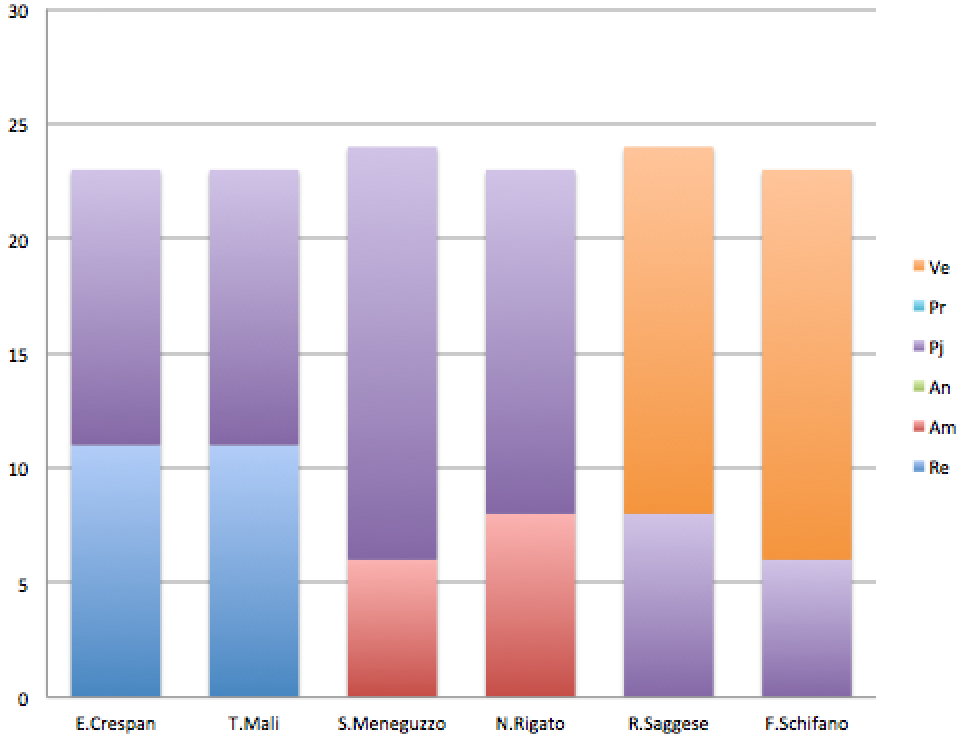
\includegraphics[scale=0.65]{img/fig3.png}
  \captionof{figure}{Incidenza ore per ruolo, Progettazione architetturale}
\end{center}

\subsection{Progettazione in Dettaglio}
Nell’attività di Progettazione in dettaglio ciascun componente dovrà rivestire i seguenti ruoli:
\begin{center}
  \centering
  \begin{tabular} {|c|c|c|c|c|c|c|c|}
    \hline
    \textbf{Nominativo} & \multicolumn{6}{|c|}{\textbf{Ore per ruolo}} & \textbf{Ore Totali} \\
    & \textbf{Re} & \textbf{Am} & \textbf{An} & \textbf{Pj} & \textbf{Pr} & \textbf{Ve} & \\
    \hline
    Emanuele Crespan & & & &11 & &12 &23\\
    \hline
    Tomas Mali & &12 & &11 & & &23\\
    \hline
    Silvio Meneguzzo & & & &9 & &13 &22\\
    \hline
    Nicolò Rigato & & & &11 & &11 &22\\
    \hline
    Riccardo Saggese &9 & & &14 & & &23\\
    \hline
    Federica Schifano &8 & & &14 & & &22\\
    \hline
  \end{tabular}
  \captionof{table}{Ore per componente, Progettazione in Dettaglio}
  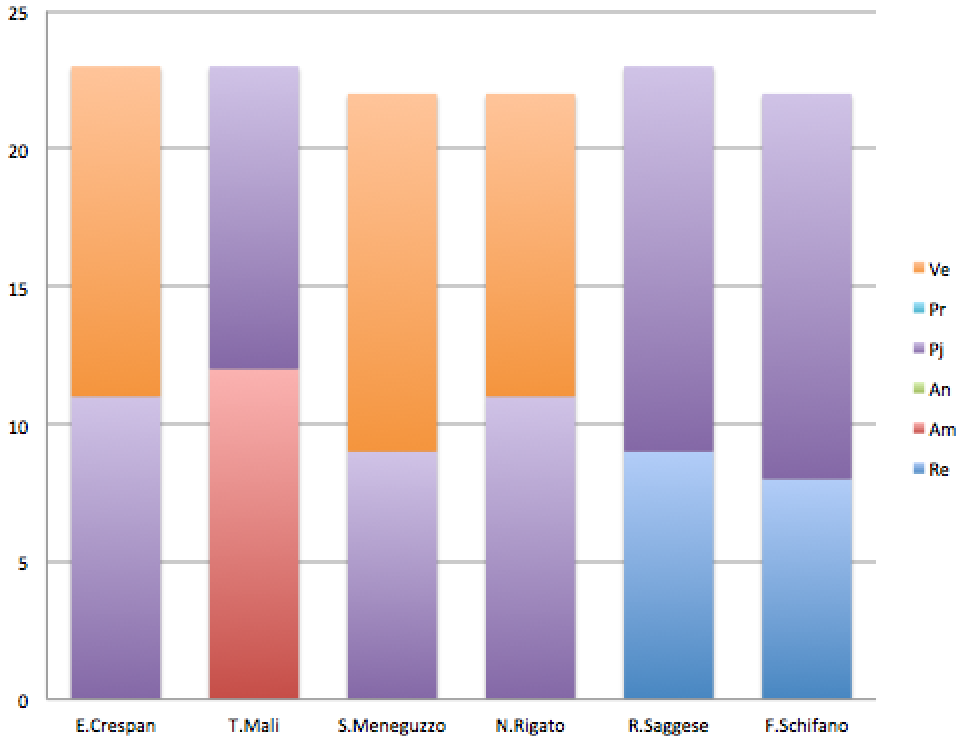
\includegraphics[scale=0.65]{img/fig4.png}
  \captionof{figure}{Incidenza ore per ruolo, Progettazione in Dettaglio}
\end{center}

\subsection{Codifica}
Nell’attività di Codifica ciascun componente dovrà rivestire i seguenti ruoli:
\begin{center}
  \centering
  \begin{tabular} {|c|c|c|c|c|c|c|c|}
    \hline
    \textbf{Nominativo} & \multicolumn{6}{|c|}{\textbf{Ore per ruolo}} & \textbf{Ore Totali} \\
    & \textbf{Re} & \textbf{Am} & \textbf{An} & \textbf{Pj} & \textbf{Pr} & \textbf{Ve} & \\
    \hline
    Emanuele Crespan & & & &6 &21 &10 &37\\
    \hline
    Tomas Mali & & & &7 &20 &10 &37\\
    \hline
    Silvio Meneguzzo &6 & & & &19 &11 &36\\
    \hline
    Nicolò Rigato &7 & & & &20 &10 &37\\
    \hline
    Riccardo Saggese & & & &7 &18 &11 &36\\
    \hline
    Federica Schifano & &6 & & &20 &11 &37\\
    \hline
  \end{tabular}
  \captionof{table}{Ore per componente, Codifica}
  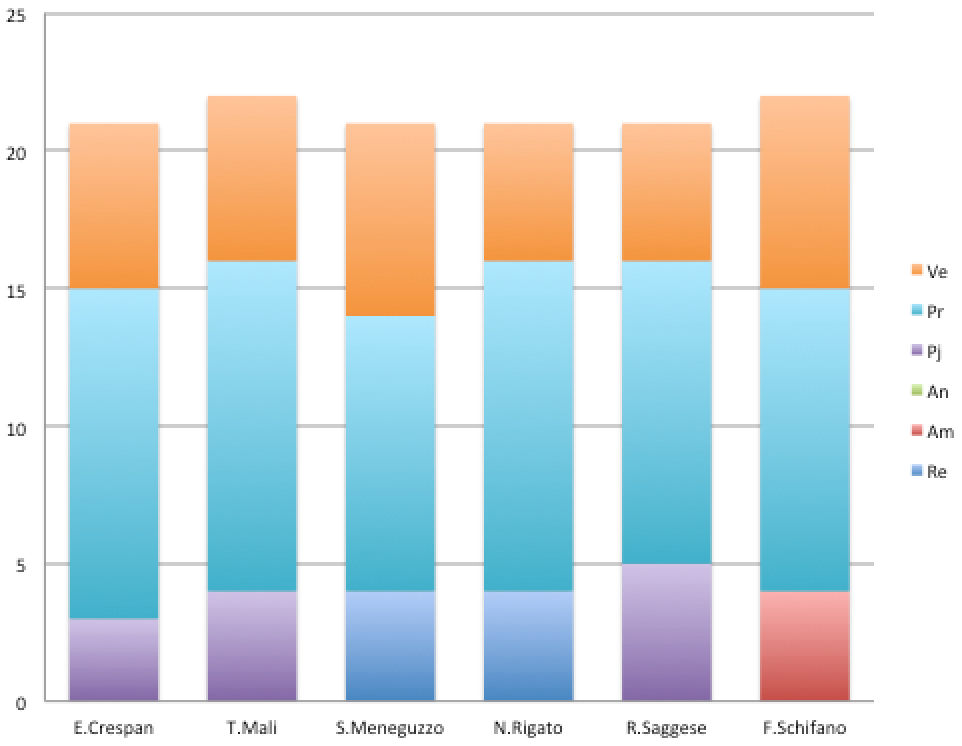
\includegraphics[scale=0.65]{img/fig5.png}
  \captionof{figure}{Incidenza ore per ruolo, Codifica}
\end{center}

\subsection{Validazione}
Nell’attività di Validazione ciascun componente dovrà rivestire i seguenti ruoli:
\begin{center}
  \centering
  \begin{tabular} {|c|c|c|c|c|c|c|c|}
    \hline
    \textbf{Nominativo} & \multicolumn{6}{|c|}{\textbf{Ore per ruolo}} & \textbf{Ore Totali} \\
    & \textbf{Re} & \textbf{Am} & \textbf{An} & \textbf{Pj} & \textbf{Pr} & \textbf{Ve} & \\
    \hline
    Emanuele Crespan &9 & & &5 & &10 &24\\
    \hline
    Tomas Mali &9 & & & 6& &9 &24\\
    \hline
    Silvio Meneguzzo & & & &6 & &18 &24\\
    \hline
    Nicolò Rigato & & & &6 & &18 &24\\
    \hline
    Riccardo Saggese &8 & & &6 & &10 &24\\
    \hline
    Federica Schifano & & & &6 & &18 &24\\
    \hline
  \end{tabular}
  \captionof{table}{Ore per componente, Validazione}
  5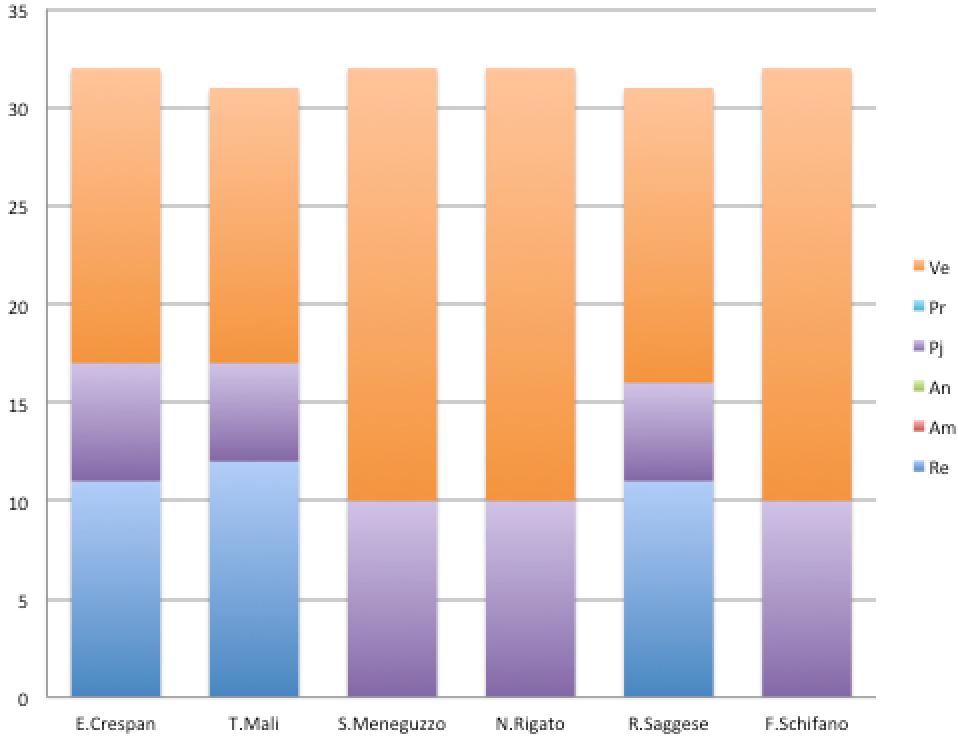
\includegraphics[scale=0.65]{img/fig6.png}
  \captionof{figure}{Incidenza ore per ruolo, Validazione}
\end{center}

\subsection{Totali}
La tabella seguente illustra le ore totali che ogni componente dedicherà per il progetto, mettendo in evidenza anche quelle che verranno poi rendicontate.\\ \\


\begin{center}
	\begin{tabular}{|c|c|c|c|c|c|c|c|c|}
		\hline
		\multirow{2}{*}{\textbf{Nominativo}} & & \multicolumn{6}{c|}{\textbf{Ore per ruolo}} & \multirow{2}{*}{\textbf{Ore totali}} \\
		& & \textbf{Re} & \textbf{Am} & \textbf{An} & \textbf{Pj} & \textbf{Pr} & \textbf{Ve} & \\
		\hline
		\hline
		\multirow{2}{*}{E.Crespan}		&	Rendicontate	&	20	&	0	&	0	&	34	&	21	& 32 	&	107	\\
		\cline{2-9}
		&	Totali			&	20	&	25	&	23	&	34	&	21	& 	32	&	155	\\
		\hline
		\hline
		\multirow{2}{*}{T.Mali}	&	Rendicontate	&	20	&	12	&	0	&	36	&	20	&  19	&	107	\\
		\cline{2-9}
		&	Totali			&	30	&	17	&	14	&	36	&	20	& 	39	&	156	\\
		\hline
		\hline
		\multirow{2}{*}{S.Meneguzzo}	&	Rendicontate	&	6	&	6	&	0	&	33	&	19	&	42	&	106	\\
		\cline{2-9}
		&	Totali			&	6	&	6	&	22	&	33	&	19	&	68	&	154	\\
		\hline
		\hline
		\multirow{2}{*}{N.Rigato}	&	Rendicontate	&	7	&	8	&	0	&	32	&	20	&	39	&	106	\\
		\cline{2-9}
		&	Totali			&	37	&	8	&	19	&	32	&	20	&	39	&	155	\\
		\hline
		\hline
		\multirow{2}{*}{R.Saggese}		&	Rendicontate	&	17	&	0	&	0	&	35	&	18	& 	37	&	107	\\
		\cline{2-9}
		&	Totali			&	17	&	10	&	18	&	35	&	18	& 	57	&	155	\\
		\hline
		\hline
		\multirow{2}{*}{F.Schifano}	&	Rendicontate	&	8	&	6	&	0	&	26	&	20	& 	46	&	106	\\
		\cline{2-9}
		&	Totali			&	28	&	6	&	18	&	26	&	20	& 	57	&	155	\\
		\hline
		
	\end{tabular}
	\captionof{table}{Ore per componente per ruolo, rendicontate e totali}
\end{center}

\section{Prospetto economico}
In questa sezione vengono presentate, per ciascun periodo del progetto, le ore di impegno calcolate
a preventivo per i ruoli coinvolti, divise tra ore di investimento e ore contabilizzate. Si ricorda che
il periodo di Analisi dei Requisiti non è a carico del \glossario{committente} e quindi non sarà considerato
nel calcolo del preventivo, ma solo indicato come risorsa di investimento.

\subsection{Analisi dei Requisiti}
Nel periodo riguardante la fase di Analisi dei Requisiti le ore tra i ruoli sono state divise nel seguente modo: \\ \\

\begin{center}
  \centering
  \begin{tabular}{|c|c|c|}
    \hline
    \textbf{Ruolo} & \textbf{Ore} & \textbf{Costo} \\
    \hline
     \emph{Responsabile}  & 40 & 1200 \\
    \hline  \emph{Amministratore}  & 20 & 400 \\
    \hline  \emph{Analista}  & 80 & 2000 \\
    \hline  \emph{Verificatore}  & 55 & 825 \\
    \hline
    \textbf{Totale} & 195 & 4425 \\
    \hline
  \end{tabular}
  \captionof{table}{Costo per ruolo, Analisi dei Requisiti}
  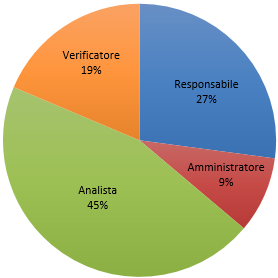
\includegraphics[scale=0.7]{img/1-AnalisiRequisiti.png}
  \captionof{figure}{Costo per ruolo, Analisi dei Requisiti}
\end{center}

\subsection{Analisi dei Requisiti in Dettaglio}
Nel periodo riguardante la fase di Analisi dei Requisiti in Dettaglio le ore tra i ruoli sono state divise nel seguente modo: \\ \\

\begin{center}
  \centering
  \begin{tabular}{|c|c|c|}
    \hline
    \textbf{Ruolo} & \textbf{Ore} & \textbf{Costo} \\
    \hline
     \emph{Responsabile}  & 20 & 600 \\
    \hline  \emph{Amministratore}  & 20 & 400 \\
    \hline  \emph{Analista}  & 34 & 850 \\
    \hline  \emph{Verificatore}  & 22 & 330 \\
    \hline
    \textbf{Totale} & 96 & 2180 \\
    \hline
  \end{tabular}
  \captionof{table}{Costo per ruolo, Analisi dei Requisiti in Dettaglio}
  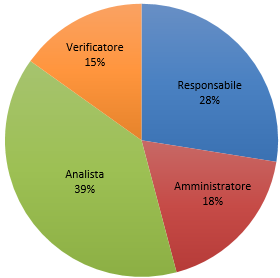
\includegraphics[scale=0.7]{img/2-AnalisiDettaglio.png}
  \captionof{figure}{Costo per ruolo, Analisi dei Requisiti in Dettaglio}
\end{center}

\subsection{Progettazione Architetturale}
Nel periodo riguardante la fase di Progettazione Architetturale le ore tra i ruoli sono state divise nel seguente modo: \\ \\

\begin{center}
  \centering
  \begin{tabular}{|c|c|c|}
    \hline
    \textbf{Ruolo} & \textbf{Ore} & \textbf{Costo} \\
    \hline
     \emph{Responsabile}  & 22 & 660 \\
    \hline  \emph{Amministratore}  & 14 & 280 \\
    \hline  \emph{Progettista}  & 71 & 1562 \\
    \hline  \emph{Verificatore}  & 33 & 495 \\
    \hline
    \textbf{Totale} & 140 & 2997 \\
    \hline
  \end{tabular}
  \captionof{table}{Costo per ruolo, Progettazione Architetturale}
  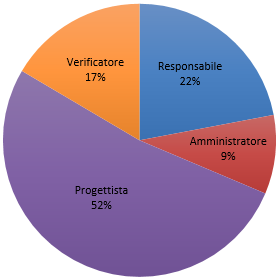
\includegraphics[scale=0.7]{img/3-ProgArchitetturale.png}
  \captionof{figure}{Costo per ruolo, Progettazione Architetturale}
\end{center}

\subsection{Progettazione di Dettaglio}
Nel periodo riguardante la fase di Progettazione di Dettaglio le ore tra i ruoli sono state divise nel seguente modo: \\ \\

\begin{center}
  \centering
  \begin{tabular}{|c|c|c|}
    \hline
    \textbf{Ruolo} & \textbf{Ore} & \textbf{Costo} \\
    \hline
     \emph{Responsabile}  & 17 & 510 \\
    \hline  \emph{Amministratore}  & 12 & 240 \\
    \hline  \emph{Progettista}  & 70 & 1540 \\
    \hline  \emph{Verificatore}  & 36 & 540 \\
    \hline
    \textbf{Totale} & 135 & 2830 \\
    \hline
  \end{tabular}
  \captionof{table}{Costo per ruolo, Progettazione di Dettaglio}
  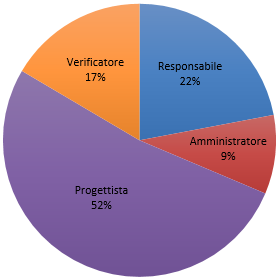
\includegraphics[scale=0.7]{img/3-ProgArchitetturale.png}
  \captionof{figure}{Costo per ruolo, Progettazione di Dettaglio}
\end{center}

\subsection{Codifica}
Nel periodo riguardante la fase di Codifica le ore tra i ruoli sono state divise nel seguente modo: \\ \\

\begin{center}
  \centering
  \begin{tabular}{|c|c|c|}
    \hline
    \textbf{Ruolo} & \textbf{Ore} & \textbf{Costo} \\
    \hline
     \emph{Responsabile}  & 13 & 390 \\
    \hline  \emph{Amministratore}  & 6 & 120 \\
    \hline  \emph{Progettista}  & 20 & 440 \\
    \hline  \emph{Programmatore}  & 118 & 1770 \\
    \hline  \emph{Verificatore}  & 63 & 945 \\
    \hline
    \textbf{Totale} & 220 & 3365 \\
    \hline
  \end{tabular}
  \captionof{table}{Costo per ruolo, Codifica}
  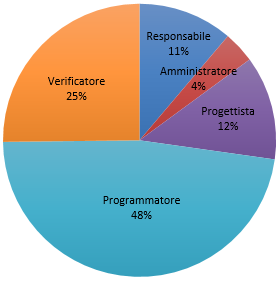
\includegraphics[scale=0.7]{img/5-Codifica.png}
  \captionof{figure}{Costo per ruolo, Codifica}
\end{center}

\subsection{Validazione}
Nel periodo riguardante la fase di Validazione le ore tra i ruoli sono state divise nel seguente modo: \\ \\

\begin{center}
  \centering
  \begin{tabular}{|c|c|c|}
    \hline
    \textbf{Ruolo} & \textbf{Ore} & \textbf{Costo} \\
    \hline
     \emph{Responsabile}  & 26 & 780 \\
    \hline  \emph{Progettista}  & 35 & 770 \\
    \hline  \emph{Verificatore}  & 83 & 1245 \\
    \hline
    \textbf{Totale} & 144 & 2795 \\
    \hline
  \end{tabular}
  \captionof{table}{Costo per ruolo, Validazione}
  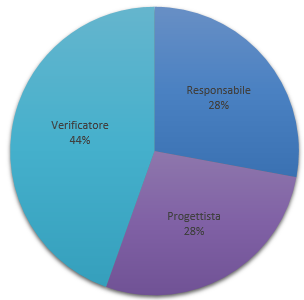
\includegraphics[scale=0.7]{img/6-Validazione.png}
  \captionof{figure}{Costo per ruolo, Validazione}
\end{center}

\subsection{Totale}
\subsubsection{Ore totali}
Le ore totali, previste per la realizzazione dell’intero progetto, comprese le ore di investimento,sono riportate nella tabella seguente: \\ \\

\begin{center}
  \centering
  \begin{tabular}{|c|c|c|c|}
    \hline
    \textbf{Ruolo} & \textbf{Ore} & \textbf{Ore remunerabili} & \textbf{Costo} \\
    \hline  \emph{Responsabile}  & 138 & 78 & 2340 \\
    \hline  \emph{Amministratore}  & 72 & 32 & 640 \\
    \hline  \emph{Analista}  & 114 & 0 & 0 \\
    \hline  \emph{Progettista}  & 196 & 196 & 4312 \\
    \hline  \emph{Programmatore}  & 118 & 118 & 1770 \\
    \hline  \emph{Verificatore}  & 292 & 215 & 3225 \\
    \hline
    \textbf{Totale} & 930 & 639 & 12287 \\
    \hline
  \end{tabular}
  \captionof{table}{Costo totale per ruolo}
  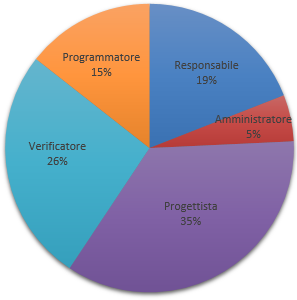
\includegraphics[scale=0.7]{img/7-Totale.png}
  \captionof{figure}{Costo totale per ruolo}
\end{center}

\subsubsection{Conclusioni}

Il costo totale del progetto, indicato nella tabella 20, è di € 12.287.

\section{Consuntivo di periodo}

Verranno elencate di seguito le spese effettivamente sostenute, relative alle spese totali, sia per ruolo che per persone.

Sarà infine presentato un bilancio:
\begin{itemize}
\item Positivo: se il preventivo supera il consuntivo
\item Negativo: se il consuntivo supera il preventivo
\item In pari: se consuntivo e preventivo si equivalgono
\end{itemize}

\subsection{Analisi dei Requisiti}

\subsubsection{Consuntivo}

Verranno indicate le ore di ruolo e le spese effettivamente sostenute nella fase di Analisi dei Requisiti. Questi dati sono quindi relativi alle ore totali di investimento.

\begin{center}
  \centering
  \begin{tabular}{|c|c|c|}
    \hline
    \textbf{Ruolo} & \textbf{Ore} & \textbf{Costo} \\
    \hline
     \emph{Responsabile}  & 40 & 1200 \\
    \hline  \emph{Amministratore}  & 20 & 400 \\
    \hline  \emph{Analista}  & 80 & 2000 \\
    \hline  \emph{Verificatore}  & 55 & 825 \\
    \hline
    \textbf{Totale consuntivo} & 195 & 4425 \\
    \hline
    \textbf{Totale preventivo} & 195 & 4425 \\
    \hline
    \textbf{Totale differenza} & - & - \\
    \hline
  \end{tabular}
  \captionof{table}{Ore totali di investimento - differenza preventivo/consuntivo in fase di Analisi dei Requisiti}

\end{center}

\subsubsection{Conclusioni}

Il team non ha impiegato un numero di risorse diverso da quello previsto. Di conseguenza, per questa fase, non sono emerse differenze tra il consuntivo e il preventivo lasciando il bilancio complessivo in pari.


\subsection{Analisi di dettaglio}

\subsubsection{Consuntivo}

Verranno indicate le ore di ruolo e le spese effettivamente sostenute nella fase di Analisi di dettaglio. Questi dati sono quindi relativi alle ore totali di investimento.

\begin{center}
	\centering
	\begin{tabular}{|c|c|c|}
		\hline
		\textbf{Ruolo} & \textbf{Ore} & \textbf{Costo} \\
		\hline
		\emph{Responsabile}  & 20 & 600 \\
		\hline  \emph{Amministratore}  & 20 & 400 \\
		\hline  \emph{Analista}  &  34 &850  \\
		\hline  \emph{Verificatore} & 22(-1)  &315  \\
		\hline
		\textbf{Totale consuntivo} &  95 & 2165  \\
		\hline
		\textbf{Totale preventivo} &  96&  2180\\
		\hline
		\textbf{Totale differenza} & -1 & -15 \\
		\hline
	\end{tabular}
	\captionof{table}{Ore totali di investimento - differenza preventivo/consuntivo in fase di Analisi di dettaglio}
	
\end{center}

\subsubsection{Conclusioni}

Il team ha impiegato un numero di risorse inferiore rispetto a quello previsto per il ruolo di Verificatore. Di conseguenza, per questa fase, sono emerse piccole differenze tra il consuntivo e il preventivo provocando così un risparmio di: -15€.
Ricordiamo che i dati riportati fino a questo punto sono a scopo informativo in quanto
le fasi di Analisi dei Requisiti e Analisi di Dettaglio non vengono poste a carico del Committente.


\subsection{Progettazione Architetturale}

\subsubsection{Consuntivo}

Verranno indicate le ore di ruolo e le spese effettivamente sostenute nella fase di Progettazione architetturale. Questi dati sono quindi relativi alle ore totali di investimento.

\begin{center}
	\centering
	\begin{tabular}{|c|c|c|}
		\hline
		\textbf{Ruolo} & \textbf{Ore} & \textbf{Costo} \\
		\hline
		\emph{Responsabile}  & 22(-1) & 630 \\
		\hline  \emph{Amministratore}  & 14(-1) & 260 \\
		\hline  \emph{Progettista}  & 71(+3) & 1628 \\
		\hline  \emph{Verificatore}  & 33(-1) & 510 \\
		\hline
		\textbf{Totale consuntivo} & 140 & 3028 \\
		\hline
		\textbf{Totale preventivo} & 140 & 2997 \\
		\hline
		\textbf{Totale differenza} & 0 & +31 \\
		\hline
	\end{tabular}
	\captionof{table}{Ore totali di investimento - differenza preventivo/consuntivo in fase di Progettazione architetturale}
	
\end{center}

\subsubsection{Conclusioni}

Il team ha impiegato un numero di risorse diverso da quello previsto. Sono emerse alcune differenze con il preventivo: una diminuzione per i ruoli di Responsabile, Amministratore e Verificatore, ed una maggiorazione per quelli di Progettista. Di conseguenza, per questa fase, sono emerse differenze tra il consuntivo e il preventivo per una perdita di: +31€.

\subsubsection{Preventivo a finire}
Da quanto si evince dal consuntivo corrente per questo periodo, il team ha superato il preventivo
di 31€. Considerando i 15€ risparmiati nella fase precedente il bilancio è in negativo di 16€. Obelix si impegna prendendosi a carico le spese che eccedono dal preventivo. 

\subsection{Progettazione in Dettaglio}

\subsubsection{Consuntivo}

Verranno indicate le ore di ruolo e le spese effettivamente sostenute nella fase di Progettazione in Dettaglio. Questi dati sono quindi relativi alle ore totali di investimento.

\begin{center}
	\centering
	\begin{tabular}{|c|c|c|}
		\hline
		\textbf{Ruolo} & \textbf{Ore} & \textbf{Costo} \\
		\hline
		\emph{Responsabile}  & 17(+1) & 540 \\
		\hline  \emph{Amministratore}  & 12(-1) & 220 \\
		\hline  \emph{Progettista}  & 70(+2) & 1588 \\
		\hline  \emph{Verificatore}  & 36 & 540 \\
		\hline
		\textbf{Totale consuntivo} & 137 & 2888 \\
		\hline
		\textbf{Totale preventivo} & 135 & 2830 \\
		\hline
		\textbf{Totale differenza} & +2 & +58 \\
		\hline
	\end{tabular}
	\captionof{table}{Ore totali di investimento - differenza preventivo/consuntivo in fase di Progettazione in Dettaglio}
	
\end{center}

\subsubsection{Conclusioni}

Il team ha impiegato un numero di risorse diverso da quello previsto. Sono emerse alcune differenze con il preventivo: una diminuzione per il ruolo di Amministratore, e una maggiorazione per quelli di Progettista e Responsabile. Di conseguenza, per questa fase, sono emerse differenze tra il consuntivo e il preventivo per una perdita di: +58€.

\subsubsection{Preventivo a finire}
Da quanto si evince dal consuntivo corrente per questo periodo, il team ha superato il preventivo
di 58€. Considerando le fasi precedenti, il bilancio risulta essere in negativo di 74€. Obelix si impegna prendendosi a carico le spese che eccedono dal preventivo. 

\subsection{Codifica}

\subsubsection{Consuntivo}

Verranno indicate le ore di ruolo e le spese effettivamente sostenute nella fase di Codifica. Questi dati sono quindi relativi alle ore totali di investimento.

\begin{center}
	\centering
	\begin{tabular}{|c|c|c|}
		\hline
		\textbf{Ruolo} & \textbf{Ore} & \textbf{Costo} \\
		\hline
		\emph{Responsabile}  & 13 & 390 \\
		\hline  \emph{Amministratore}  & 6 & 120 \\
		\hline  \emph{Progettista}  & 20 & 440 \\
		\hline  \emph{Programmatore}  & 118(+3) & 1815 \\
		\hline  \emph{Verificatore}  & 638(-2) & 915 \\
		\hline
		\textbf{Totale consuntivo} & 220 & 3680 \\
		\hline
		\textbf{Totale preventivo} & 220 &  3665\\
		\hline
		\textbf{Totale differenza} & - & +15 \\
		\hline
	\end{tabular}
	\captionof{table}{Ore totali di investimento - differenza preventivo/consuntivo in fase di Codifica}
	
\end{center}
\newpage
\subsubsection{Conclusioni}

Il team ha impiegato un numero di risorse diverso da quello previsto. Sono emerse alcune differenze con il preventivo: una diminuzione per il ruolo di Verificatore e una maggiorazione per quello di Programmatore. Di conseguenza, per questa fase, sono emerse differenze tra il consuntivo e il preventivo per una perdita di: 15€.

\subsubsection{Preventivo a finire}
Da quanto si evince dal consuntivo corrente per questo periodo, il team ha superato il preventivo
di 15€. Considerando le fasi precedenti, il bilancio risulta essere in negativo di 89€. Obelix si impegna prendendosi a carico le spese che eccedono dal preventivo. 


\clearpage

\appendix
\section{Organigramma}
\subsection{Redazione}

\begin{center}
  \centering
  \begin{tabular}{|c|c|c|}
    \hline
    \textbf{Nominativo} & \textbf{Data di redazione} & \textbf{Firma} \\
    \hline
    Nicolò Rigato & 2017-02-25 & 
    \begin{minipage}{.3\textwidth}
      
\includegraphics[width=\linewidth]{../../../file_comuni/firme/nr.jpg}
    \end{minipage}
 \\\hline
  \end{tabular}
  \captionof{table}{Redazione}

\end{center}

\subsection{Approvazione}

\begin{center}
	\centering
	\begin{tabular}{|c|c|c|}
		\hline
		\textbf{Nominativo} & \textbf{Data di approvazione} & \textbf{Firma} \\
		\hline Nicolò Rigato & 2017-03-11 & 
    \begin{minipage}{.3\textwidth}
      
\includegraphics[width=\linewidth]{../../../file_comuni/firme/nr.jpg}
    \end{minipage}
 \\
		\hline Prof. Tullio Vardanega &  &  \\[40pt]\hline
	\end{tabular}
	\captionof{table}{Approvazione}
	
\end{center}

\subsection{Accettazione dei componenti}

\begin{center}
	\centering
	\begin{tabular}{|c|c|c|}
		\hline
		\textbf{Nominativo} & \textbf{Data di accettazione} & \textbf{Firma} \\
		\hline Emanuele Crespan & 2017-03-11 &  
    \begin{minipage}{.3\textwidth}
      
\includegraphics[width=\linewidth]{../../../file_comuni/firme/ec.jpg}
    \end{minipage}\\
		\hline Tomas Mali & 2017-03-11 & 
    \begin{minipage}{.3\textwidth}
      
\includegraphics[width=\linewidth]{../../../file_comuni/firme/tm.jpg}
    \end{minipage} \\
		\hline Silvio Meneguzzo & 2017-03-11 &    
 \begin{minipage}{.3\textwidth}
      
\includegraphics[width=\linewidth]{../../../file_comuni/firme/sm.jpg}
    \end{minipage} \\
		\hline Nicolò Rigato & 2017-03-11 & 
    \begin{minipage}{.3\textwidth}
      
\includegraphics[width=\linewidth]{../../../file_comuni/firme/nr.jpg}
    \end{minipage} \\
		\hline Riccardo Saggese & 2017-03-11 &      
\begin{minipage}{.3\textwidth}
      
\includegraphics[width=\linewidth]{../../../file_comuni/firme/rs.jpg}
    \end{minipage}
\\
		\hline Federica Schifano & 2017-03-11 & 
    \begin{minipage}{.3\textwidth}
      
\includegraphics[width=\linewidth]{../../../file_comuni/firme/fs.jpg}
    \end{minipage}
 \\\hline
	\end{tabular}
	\captionof{table}{Accettazione}
	
\end{center}
\clearpage
\subsection{Componenti}

\begin{center}
	\centering
%\small
  \begin{turn}{90}
\begin{tabular}{|c|c|c|c|}
%*{1}{>{\centering\arraybackslash}p{1.3cm}|}
%*{1}{>{\centering\arraybackslash}p{1.5cm}|}
%*{1}{>{\centering\arraybackslash}p{6 cm}|}
%*{1}{>{\centering\arraybackslash}p{1.6 cm}|}}
   \hline
		\textbf{Nominativo} & \textbf{Matricola} & \textbf{Indirizzo di posta elettronica} & \textbf{Ruoli}\\

		\hline \makecell{Emanuele \\ Crespan} & 1004994 & emanuele.crespan@gmail.com & \makecell{ \emph{Amministratore} \\Analista} \\
		\hline \makecell{Tomas \\ Mali} & 1077040 & tomas.mali@studenti.unipd.it & \makecell{ \emph{Amministratore} \\ \emph{Analista} \\Verificatore} \\
		\hline \makecell{Silvio \\ Meneguzzo} & 1097458 & silvio.meneguzzo@studenti.unipd.it & \makecell{ \emph{Analista} \\Verificatore} \\
		\hline \makecell{Nicolò \\ Rigato} & 1006492 & nicolo.rigato.1@studenti.unipd.it & \makecell{ \emph{Responsabile} \\Analista} \\
		\hline \makecell{Riccardo \\ Saggese} & 1051333 &  riccardoalessandro.saggesecompri@studenti.unipd.it & \makecell{ \emph{Analista} \\Verificatore} \\
		\hline \makecell{Federica \\ Schifano} & 1099511 &  federica.schifano@studenti.unipd.it & \makecell{ \emph{Responsabile} \\ Analista} \\\hline
\end{tabular}

	\end{turn}
\captionof{table}{Accettazione}
	
	
\end{center}

